%%%%%%%%%%%%%%%%%%%%%%%%%%%%%%%%%%%%%%%%%
% University/School Laboratory Report
% LaTeX Template
% Version 3.1 (25/3/14)
%
% This template has been downloaded from:
% http://www.LaTeXTemplates.com
%
% Original author:
% Linux and Unix Users Group at Virginia Tech Wiki 
% (https://vtluug.org/wiki/Example_LaTeX_chem_lab_report)
%
% License:
% CC BY-NC-SA 3.0 (http://creativecommons.org/licenses/by-nc-sa/3.0/)
%
%%%%%%%%%%%%%%%%%%%%%%%%%%%%%%%%%%%%%%%%%

%----------------------------------------------------------------------------------------
%	PACKAGES AND DOCUMENT CONFIGURATIONS
%----------------------------------------------------------------------------------------

\documentclass{article}

\usepackage[version=3]{mhchem} % Package for chemical equation typesetting
\usepackage{siunitx} % Provides the \SI{}{} and \si{} command for typesetting SI units
\usepackage{graphicx} % Required for the inclusion of images
\usepackage{natbib} % Required to change bibliography style to APA
\usepackage{amsmath} % Required for some math elements 
\usepackage[table,xcdraw]{xcolor}
\usepackage{listings}
\usepackage{hyperref}
\usepackage{xcolor}
\lstset { %
    language=C++,
    backgroundcolor=\color{black!5}, % set backgroundcolor
    basicstyle=\footnotesize,% basic font setting
    numbers=left,
    stepnumber=1,
    tabsize = 2
}

\usepackage[utf8]{inputenc} %Türkçe karakterler
\usepackage{floatrow}
\usepackage{geometry}
\usepackage{caption}
\usepackage{subcaption}
\geometry{margin=1in}

\renewcommand{\lstlistingname}{Code Snippet}

%\setlength\parindent{0pt} % Removes all indentation from paragraphs

% Table float box with bottom caption, box width adjusted to content
\newfloatcommand{capbtabbox}{table}[][\FBwidth]


\renewcommand{\labelenumi}{\alph{enumi}.} % Make numbering in the enumerate environment by letter rather than number (e.g. section 6)

%\usepackage{times} % Uncomment to use the Times New Roman font

%----------------------------------------------------------------------------------------
%	DOCUMENT INFORMATION
%----------------------------------------------------------------------------------------

\title{Assignment 1: \\ Image Filtering and Hybrid Images\\ COMP 408} % Title

\author{Ahmet \textsc{Uysal}} % Author name

\date{\today} % Date for the report

\begin{document}

\maketitle % Insert the title, author and date

\begin{center}
\begin{tabular}{l r}
%Date Performed: & October 10, 2018 \\ % Date the experiment was performed
% Partners: & James Smith \\ & Mary Smith \\
Instructor: & Y\"ucel  \textsc{Yemez} % Instructor/supervisor
\end{tabular}
\end{center}

% If you wish to include an abstract, uncomment the lines below
% \begin{abstract}
% Abstract text
% \end{abstract}

%----------------------------------------------------------------------------------------
%	SECTION 1
%----------------------------------------------------------------------------------------

\section{Implementing myFilter Method}	


If f[m,n] is an image and h[i,j] is a box filter with size 2k+1 x 2l+1, then we can calculate the resulting image g[m,n] as
\begin{equation}
g[m,n] =\sum\limits_{i=-k}^k \sum\limits_{j = -l }^l h[i+k, j+l] \times f[m+i, n+j]
\end{equation}

So, by iterating over each pixel of the image and element-wise multiplying the corresponding part of the image with filter, we can calculate the resulting filtered image. However, we need to be careful at the boundaries of the image since some of the pixels we are trying to reach will not be in the image. We will solve this problem on later sections according to three different approaches: copying edge ,reflecting across edge, and zero-padding.

In addition, we are using images with three channels. So, we will have to calculate the result for each channel separately.


\subsection{Implementation using C++ and OpenCV}

Mat objects from the assignment are type CV\_64FC3, which means 64-bit floating point (double), three channeled image.

\begin{figure}[!htb]
\centering
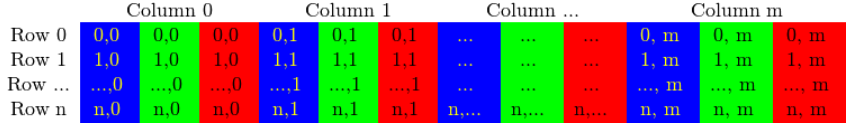
\includegraphics[width=0.9\textwidth]{multichannel.png}
\caption{OpenCV array representation in C++ for BGR color system according to official documents.}
\end{figure}

So, instead of iterating every pixel once we need to iterate three times, for each color value. This can be done by separating the image to channels, calculating the result for each channel and then combining them. However, we can also implement it without splitting by carefully calculating indexes when trying to get the neighbor pixels value for the same channel. My implementation uses the second approach to iterate over each color value of the image.

\newpage

Following code snippet is from my submission. However, some parts are modified for the sake of brevity.

\begin{lstlisting}[caption={My implementation of myFilter method.},captionpos=b]
Mat myFilter(Mat im, Mat filter, int borderType = Border_Constant) {
	Mat outI;
	// initilize our result with zeros
	outI = Mat::zeros(im.rows, im.cols, im.type());
	
	int filterHeight = filter.rows / 2;
	int filterWidth = filter.cols / 2;
	int numRows = im.rows;
	int numCols = im.cols;
	int channels = im.channels();

	// Mat to store the values we will multiply by filter
	Mat frame = Mat::zeros(filter.rows, filter.cols, CV_64F);

	// pointer to relevant row of image
	double* My = NULL;
	
	int indexX, indexY; 

  // Note that we have to separate different channels and combine them together
	// We can handle this by locating neighbor pixels on distance 3 instead of 1
	for (int m = 0; m < numRows; m++) {
		for (int n = 0; n < numCols * channels; n++) {
			for (int j = -filterHeight; j <= filterHeight; j++) {
				indexY = m + j;
				if (indexY < 0 || indexY >= numRows) {
          // Handle boundaries
				}
				My = im.ptr<double>(indexY);
				for (int i = -filterWidth; i <= filterWidth; i++) {
					indexX = n + i * channels;
					if (indexX < 0 || indexX >= numCols * channels) {
						// Handle boundaries
					}
					frame.at<double>(j + filterHeight, i + filterWidth) = My[indexX];
				}
			}
			multiply(filter, frame, frame);
			// need to specify index since method does not assume our input is one channel
			outI.ptr<double>(m)[n] = sum(frame)[0];
		}
	}
	return outI;
}
\end{lstlisting}

I used multiply and sum methods from OpenCV library. Multiply is used for element-wise multiplication of the current frame of the image being iterated and filter. Sum method returns the sum of all elements in the given matrix.

\newpage

\subsection{Boundary Problem}

To solve boundary problem, we will update our index to get value according to given border type. In the case of zero-padding (Border\_Constant), we will use boolean values to indicate whether or not we should put zero. Also, we need to check indicator before getting the pointer for My to avoid null pointer exception.

\begin{lstlisting}[caption={Boundary check for indexX (row index).},captionpos=b]
indicatorY = false;
if (indexY < 0 || indexY >= numRows) {
    if (borderType == Border_Replicate) {
        if (indexY < 0) {
            indexY = 0;
        }
        else {
            indexY = numRows - 1;
        }
    }
    else if (borderType == Border_Reflect) {
        if (indexY < 0) {
            indexY = -indexY - 1;
        }
        else {
            indexY =  2 * numRows - 1  - indexY;
        }
    }
    else {
        // make indicator true to indicate we will put 0 to frame array
        indicatorY = true;
    }
}
if (!indicatorY)
    My = im.ptr<double>(indexY);
\end{lstlisting}

\begin{lstlisting}[caption={Boundary check for indexY (column index).},captionpos=b]
indicatorX = false;
if (indexX < 0 || indexX >= numCols * channels) {
	if (borderType == Border_Replicate) {
		if (indexX < 0) {
			indexX = indexX % channels;
		}
	else {
		indexX = (indexX) % channels + (numCols - 1) * channels;
	}
}
else if (borderType == Border_Reflect) {
	if (indexX < 0) {
		indexX = (indexX % channels) + ((indexX + 1) / -channels) * channels;
	}
	else {
		indexX = (indexX % channels) + (numRows - 1) * channels 
				- ((indexX - numRows) / channels) * channels;
	}
else {
	// make indicator true to indicate we will put 0 to frame array
	indicatorX = true;
}
\end{lstlisting}


\begin{lstlisting}[caption={We should also add this check to our code from previous section.},captionpos=b]
if (indicatorX || indicatorY) {
    frame.at<double>(j + filterHeight, i + filterWidth) = 0;
}
else {
    frame.at<double>(j + filterHeight, i + filterWidth) = My[indexX];
}
\end{lstlisting}


\newpage

\subsection{Sample Results}
The results of the filtering tests are below. The order of the images are from left top to right bottom: Identity Image, Blur Image, Large Blur Image, Sobel Image, Laplacian Image, High Pass Image
\begin{figure}[!htb]
\centering
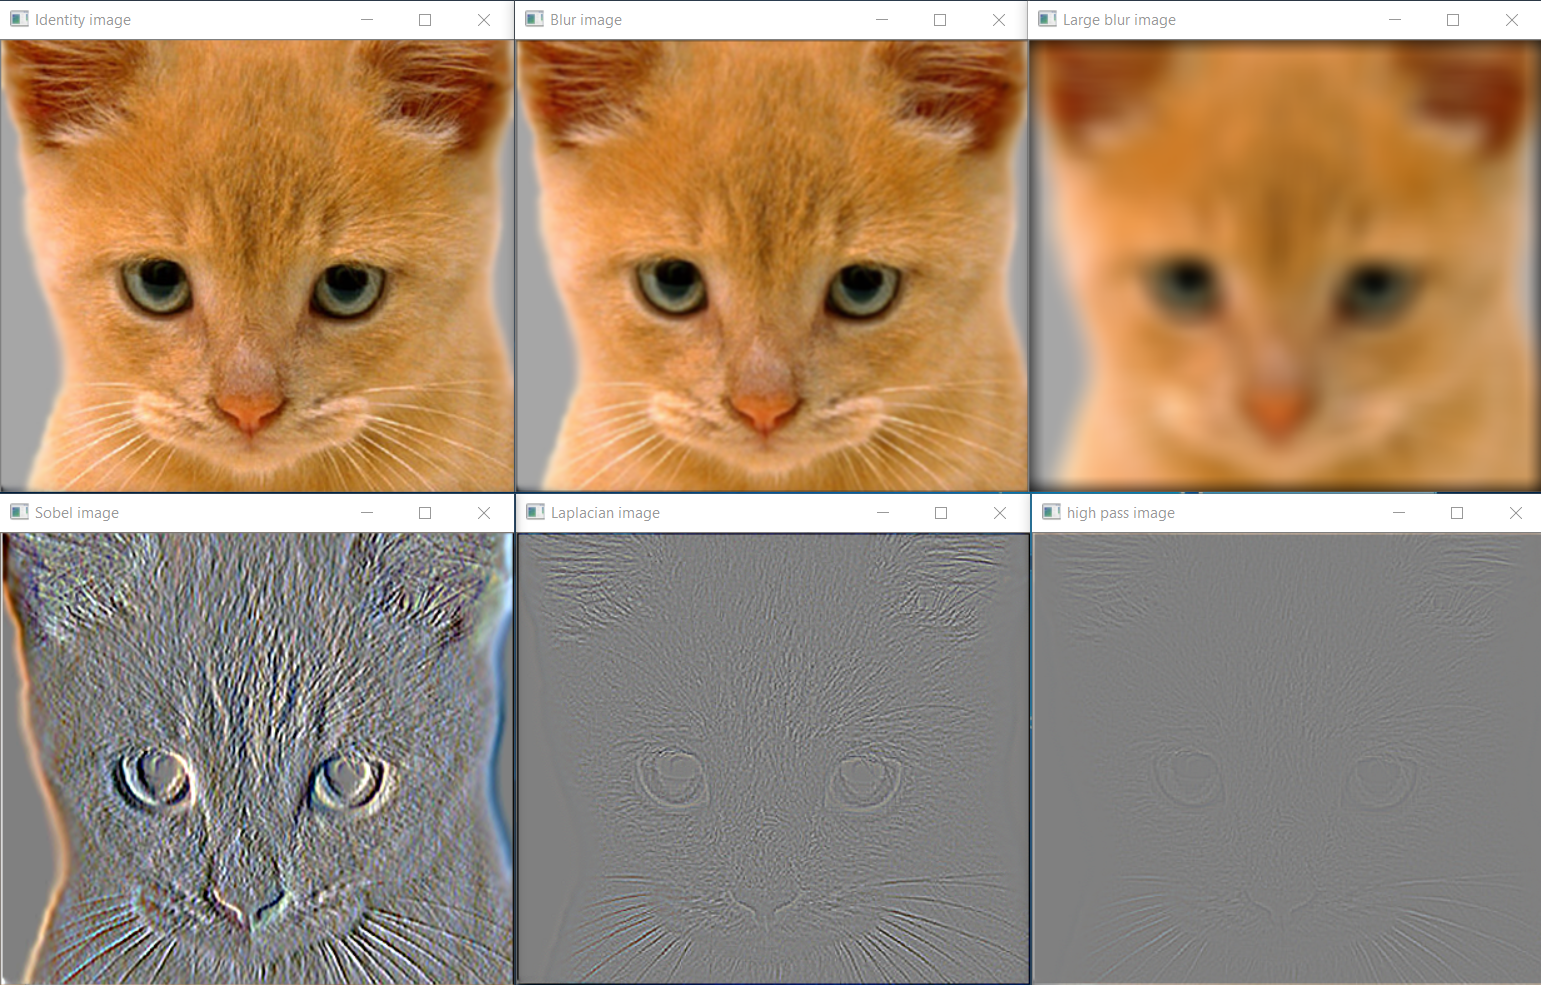
\includegraphics[width=0.75\textwidth]{cat_filtering_results.png}
\caption{Results for the filters on given cat image.}
\end{figure}


\begin{figure}[!htb]
\centering
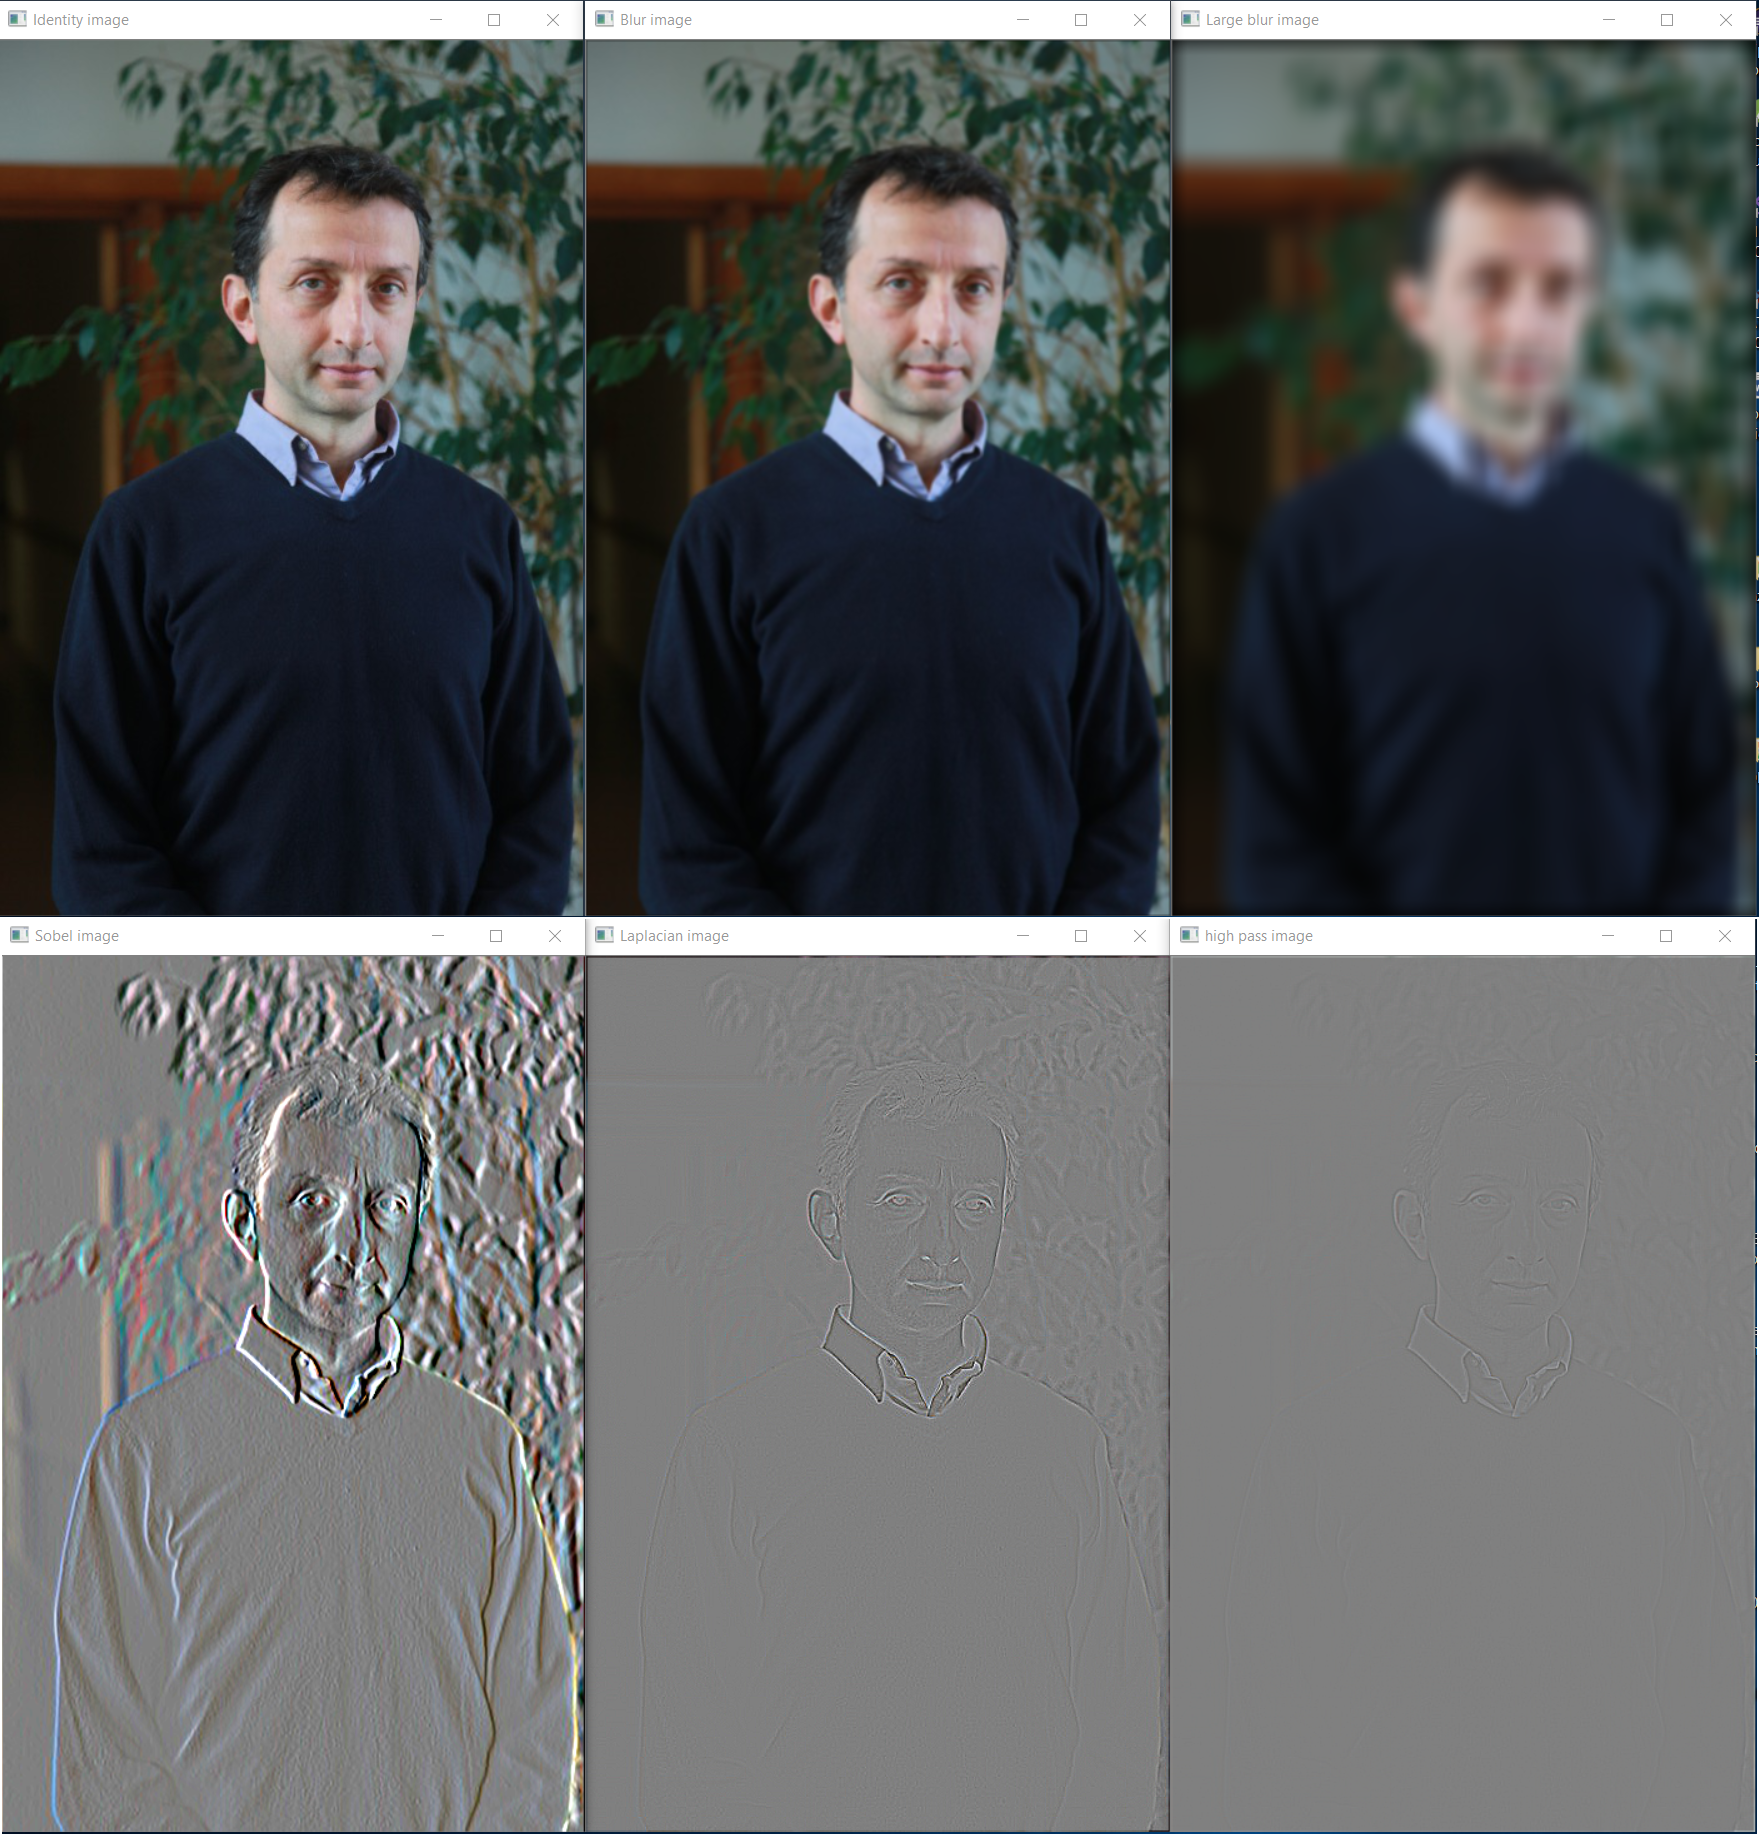
\includegraphics[width=0.6\textwidth]{yyemez_filtering_results.png}
\caption{Results for the filters on image of Prof. Y\"ucel Yemez (used with his consent).}
\end{figure}

%----------------------------------------------------------------------------------------
%	SECTION 2
%----------------------------------------------------------------------------------------

\newpage
\section{Generating the Hybrid Image }


As described in \href{http://cvcl.mit.edu/publications/OlivaTorralb_Hybrid_Siggraph06.pdf}{SIGGRAPH 2006 paper} we need to filter one of the images with low-pass filter, other image with a high-pass filter and then sum the filtered images to obtain the hybrid image.

For low-pass filtering, we will use a Gaussian filter.

For high-pass filtering, we will also use a Gaussian filter to get the low frequencies, but we will use the filtered image to subtract from the original image to get the high frequencies.

\subsection{Implementation using C++ and OpenCV}
\begin{lstlisting}[caption={Code for generating the hybrid image.},captionpos=b]
int cutoff_frequency = 7;

Mat filter = getGaussianKernel(cutoff_frequency * 4 + 1, cutoff_frequency, CV_64F);
filter = filter*filter.t();

Mat low_freq_img;
low_freq_img = myFilter(image1,filter, Border_Constant);

Mat high_freq_img;
high_freq_img = image2 - myFilter(image2, filter, Border_Constant);

Mat hybrid_image;
hybrid_image = low_freq_img + high_freq_img;

//add a scalar to high frequency image because it is centered around zero and is mostly black	
high_freq_img = high_freq_img + Scalar(0.5, 0.5, 0.5) * 255;
//Convert the resulting images type to the 8 bit unsigned integer matrix with 3 channels
high_freq_img.convertTo(high_freq_img, CV_8UC3);
low_freq_img.convertTo(low_freq_img, CV_8UC3);
hybrid_image.convertTo(hybrid_image, CV_8UC3);

Mat vis = hybrid_image_visualize(hybrid_image);

imshow("Low frequencies", low_freq_img); waitKey(0);
imshow("High frequencies", high_freq_img);	waitKey(0);
imshow("Hybrid image", vis); waitKey(0);
\end{lstlisting}

\newpage
\subsection{Sample Results}
\begin{figure}[!htb]
\begin{subfigure}{.35\textwidth}
  \centering
  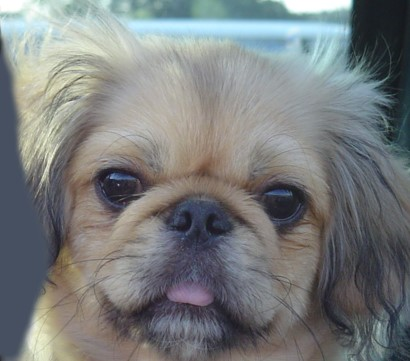
\includegraphics[width=1\textwidth]{dog.jpg}
  \caption{Original dog image.}
\end{subfigure}%
\begin{subfigure}{.35\textwidth}
  \centering
  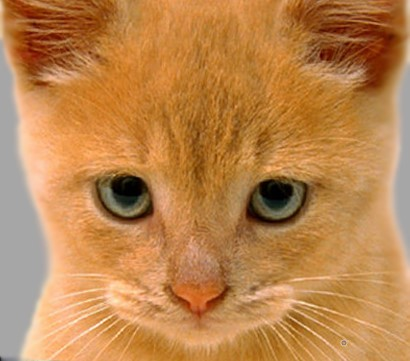
\includegraphics[width=1\textwidth]{cat.jpg}
  \caption{Original cat image.}
\end{subfigure}
\begin{subfigure}{.35\textwidth}
  \centering
  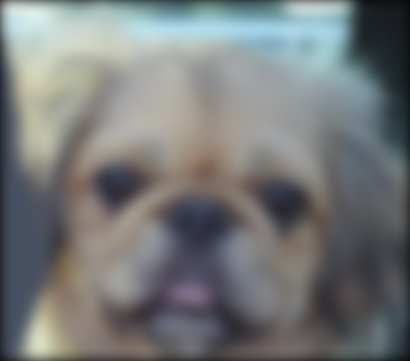
\includegraphics[width=1\textwidth]{low_frequencies.jpg}
  \caption{Low frequency component of (a).}
\end{subfigure}%
\begin{subfigure}{.35\textwidth}
  \centering
  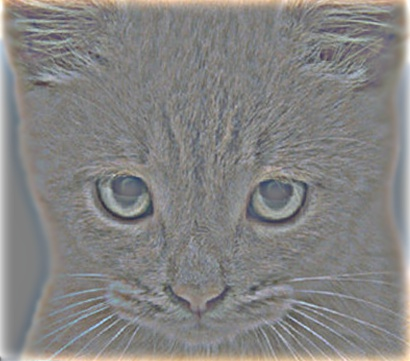
\includegraphics[width=1\textwidth]{high_frequencies.jpg}
  \caption{High frequency component of (b).}
\end{subfigure}
\begin{subfigure}{.6\textwidth}
  \centering
  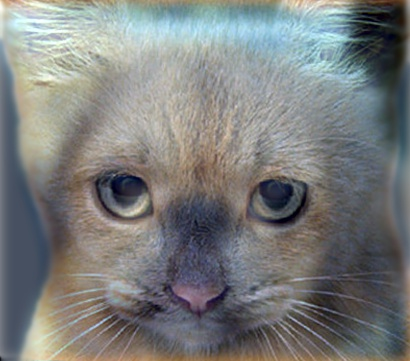
\includegraphics[width=1\textwidth]{hybrid_image.jpg}
  \caption{Hybrid image created by summing low and high frequency images.}
\end{subfigure}
\caption{Input and output images of my implementation.}
\end{figure}

\newpage

\section{DFT Spectrum}

To get the DFT Spectrum in a viewable form, we need to find the complex DFT of the image. Then, we can calculate the magnitude using

\begin{equation}
Magnitude = \sqrt{(Re(DFT(I))^2 + Im(DFT(I))^2)}
\end{equation}

In order to visualize the spectrum, we need to use logarithmic scale. So, we need to switch to logarithmic scale, i.e, log(1 + magnitude).

Finally, we need to modify the image to make origin correspond to image center for visualization purposes. 

\subsection{Implementation Using C++ and OpenCV}

\begin{lstlisting}[caption={My implementation of DTF\_Spectrum method.},captionpos=b]
Mat DFT_Spectrum(Mat img) {
	vector<Mat> im_channels(3);
	split(img, im_channels);
	img = im_channels[0];
	
	//add padding
	int optimalCol = getOptimalDFTSize(img.cols);
	int optimalRow = getOptimalDFTSize(img.rows);

	copyMakeBorder(img, img, 0, optimalRow - img.rows, 0, optimalCol - img.cols, BORDER_CONSTANT);

	//Determine complex DFT of the image.
	dft(img, img, DFT_COMPLEX_OUTPUT);
	
	Mat magI;	
	vector<Mat> im_dims(2);
	split(img, im_dims);
	// calculate the magnitude
	magnitude(im_dims[0], im_dims[1], magI);
	// add one before switching to log scale
	magI += Scalar::all(1);
	log(magI, magI);

	//crop the spectrum, if it has an odd number of rows or columns
	magI = magI(Rect(0, 0, magI.cols & -2, magI.rows & -2));
	
	// rearrange the quadrant so that the origin is at the image center
	int quadrantCols = magI.cols / 2;
	int quadrantRows = magI.rows / 2;
	Mat topLeftQuadrant(magI, Rect(0, 0, quadrantCols, quadrantRows));
	Mat topRightQuadrant(magI, Rect(quadrantCols, 0, quadrantCols, quadrantRows));
	Mat bottomLeftQuadrant(magI, Rect(0, quadrantRows, quadrantCols, quadrantRows));
	Mat bottomRightQuadrant(magI, Rect(quadrantCols, quadrantRows, quadrantCols, quadrantRows));

	// swap quadrants
	Mat tmp;                           
	topLeftQuadrant.copyTo(tmp);
	bottomRightQuadrant.copyTo(topLeftQuadrant);
	tmp.copyTo(bottomRightQuadrant);
	topRightQuadrant.copyTo(tmp);
	bottomLeftQuadrant.copyTo(topRightQuadrant);
	tmp.copyTo(bottomLeftQuadrant);

	// Transform the matrix with float values into a viewable image form.
	normalize(magI, magI, 0, 1, CV_MINMAX);
	return magI;
}
\end{lstlisting}

I implemented the method with the help of official \href{https://docs.opencv.org/2.4/doc/tutorials/core/discrete_fourier_transform/discrete_fourier_transform.html}{OpenCV Documentation on Discrete Fourier Transform.}
\newpage

\subsection{Sample Results and Conclusions}
\begin{figure}[!htb]
\begin{subfigure}{.5\textwidth}
  \centering
  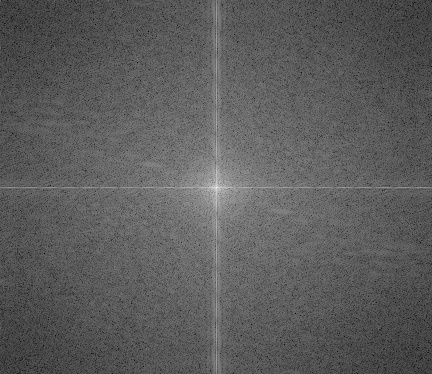
\includegraphics[width=.8\textwidth]{dog_DFT.jpg}
  \caption{DFT of original dog image.}
\end{subfigure}%
\begin{subfigure}{.5\textwidth}
  \centering
  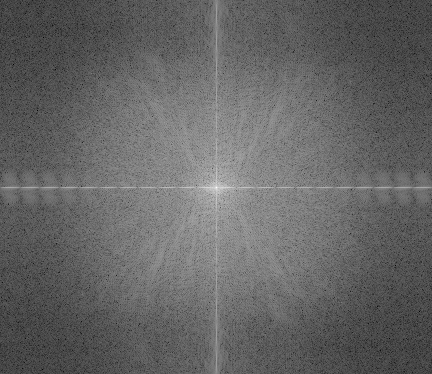
\includegraphics[width=.8\textwidth]{cat_DFT.jpg}
  \caption{DFT of original cat image.}
\end{subfigure}
\begin{subfigure}{.5\textwidth}
  \centering
  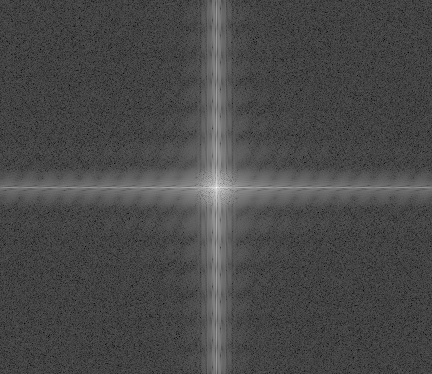
\includegraphics[width=.8\textwidth]{dog_filtered_DFT.jpg}
  \caption{DFT of low frequency component of dog.}
\end{subfigure}%
\begin{subfigure}{.5\textwidth}
  \centering
  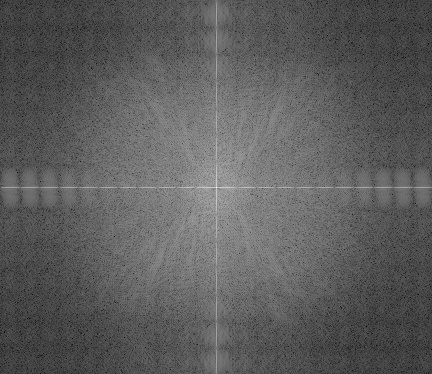
\includegraphics[width=.8\textwidth]{cat_filtered_DFT.jpg}
  \caption{DFT of high frequency component of cat.}
\end{subfigure}
\caption{DFT outputs of my implementation.}
\end{figure}

Before the filtering, both of the images have parts from almost all frequencies. However, after the filtering, DFT of dog image filtered with Gaussian filter has only frequencies below some level, its graph is confined to some small region near center. On the contrary, DFT of high frequency part of cat has lost its parts near the origin. It has only frequencies above some level.

\newpage
\section{Extra Hybrid Image}

On this last part, I wanted to try building a hybrid image myself. I used one of the portrait images of Prof. Y\"ucel with his consent. I combined his portait with one of the portraits of Amedeo Avogadro. I modified Avogadro's portait's background to minimizing unnecessary collusions. Cutoff frequency is used as 5 in the code.

\begin{figure}[!htb]
\begin{subfigure}{.4\textwidth}
  \centering
  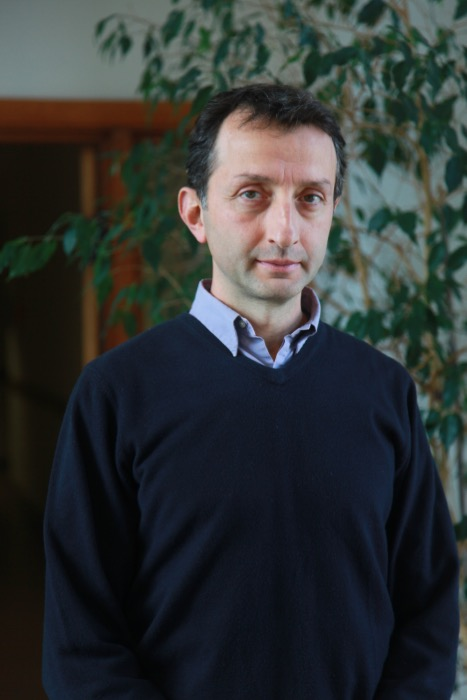
\includegraphics[width=.8\textwidth]{yyemez.jpg}
  \caption{Portrait of Prof. Y\"ucel Yemez.}
\end{subfigure}%
\begin{subfigure}{.4\textwidth}
  \centering
  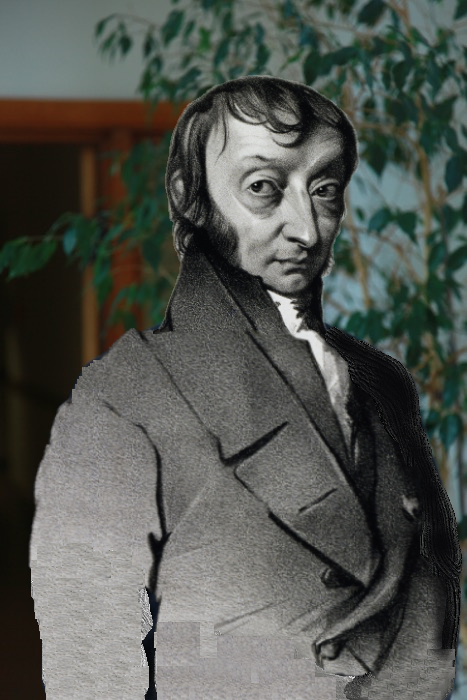
\includegraphics[width=.8\textwidth]{avogadro.png}
  \caption{Modified portraid of Amedeo Avogadro.}
\end{subfigure}
\begin{subfigure}{.4\textwidth}
  \centering
  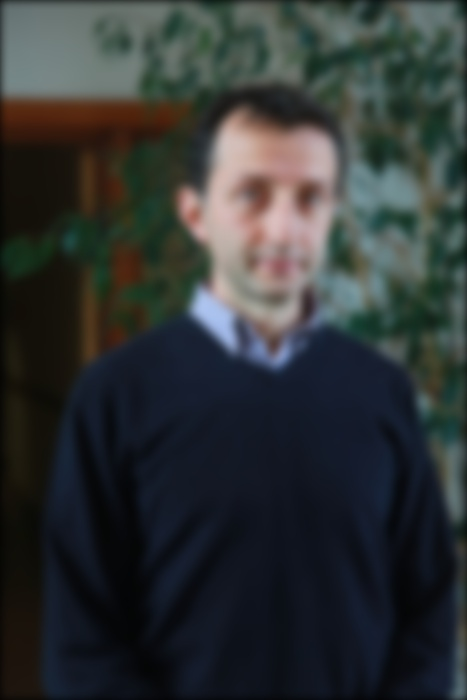
\includegraphics[width=.8\textwidth]{low_frequencies_yyemez.jpg}
  \caption{Low frequency .}
\end{subfigure}
\begin{subfigure}{.4\textwidth}
  \centering
  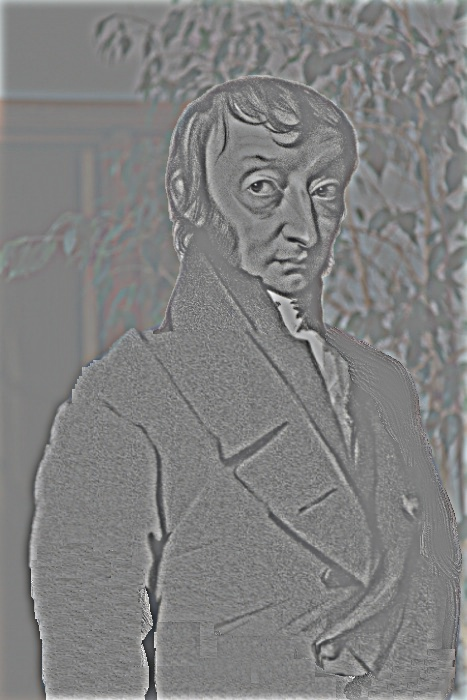
\includegraphics[width=.8\textwidth]{high_frequencies_avog.jpg}
  \caption{Modified portraid of Amedeo Avogadro.}
\end{subfigure}
\caption{Inputs to my filtered image with filtered versions.}
\end{figure}

\newpage

\begin{figure}[!htb]
\centering
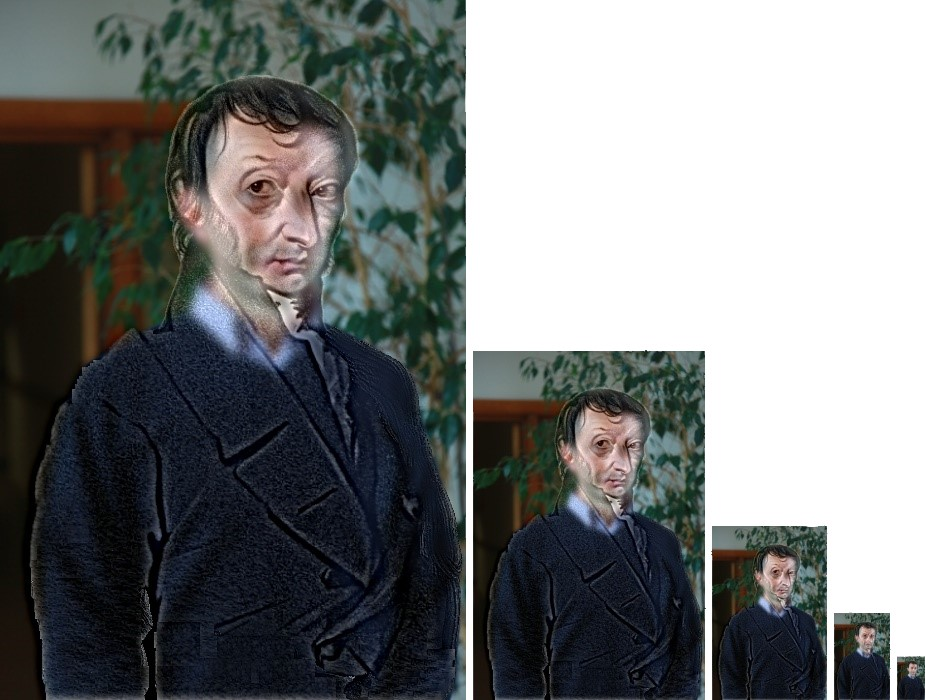
\includegraphics[width=1\textwidth]{hybrid_image_scales.jpg}
\caption{Resulting hybrid image in different scales.}
\end{figure}

\end{document}